%------- 6.1
\subsection{Definições Primitivas}
    %--- 6.1.1
    \subsubsection{Noções Primitivas}
        \begin{description}
            \item[Pontos:]
                São usado para representar localizações no espaço, mas não compreendem forma ou dimensão. Quando contidos numa mesma reta, são colineares, e quando compreendidos num mesmo plano, coplanares.
                Um conjunto de pontos quaisquer é denominado figura, e se todos os pontos que a formam forem coplanares, a figura é dita plana. \eg
                \begin{center}
                    
\begin{tikzpicture}
                        \tkzDefPoints{0/0/O, 4/4/L}
                        
                        \tkzDefPoint(1.5,1.3){A}
                        \tkzDefPoint(1,2){B}
                        \tkzDefPoint(2.2,3){C}
                        \tkzDefPoint(3.2,3){D}
                        \tkzDefPoint(2.9,2){E}
                        
                        \tkzLabelPoint[below](A){$A$}
                        \tkzLabelPoint[below left](B){$B$}
                        \tkzLabelPoint[above](C){$C$}
                        \tkzLabelPoint[below right](D){$D$}
                        \tkzLabelPoint[below](E){$E$}
                        
                        \tkzDrawPoints(A,B,C,D,E)
                        \tkzDrawPolygon(A,B,C,D,E)
                    \end{tikzpicture}    
                \end{center}
            \item[Retas:]
                São um conjunto de pontos compreendidos numa linha infinita que não faz curvas e existe em uma dimensão. Retas são ditas concorrentes se tiverem um único ponto em comum. \eg
                \begin{center}
                    \begin{tikzpicture}
                        \tkzDefPoints{0/0/O, 4/4/L}
                        
                        \tkzDefPoint(1,2){A}
                        \tkzDefPoint(3,2.5){B}
                        \tkzDefPoint(1.5,2.5){C}
                        \tkzDefPoint(3.5,1.5){D}
                        
                        \tkzLabelPoint[below](A){$A$}
                        \tkzLabelPoint[above](B){$B$}
                        \tkzLabelPoint[above](C){$C$}
                        \tkzLabelPoint[below](D){$D$}
                        
                        \tkzDrawPoints(A,B,C,D)
                        \tkzDrawLine[arrows=<->](A,B)
                        \tkzDrawLine[arrows=<->](C,D)

                        \tkzInterLL(A,B)(C,D) \tkzGetPoint{P}
                        \tkzLabelPoint[above, color=red](P){$P$}
                        \tkzDrawPoints[color=red](P)
                    \end{tikzpicture}    
                \end{center}
            \item[Planos:]
                São um conjunto de retas paralelas e perpendiculares postas lado a lado, compreendendo uma forma de duas dimensões. \eg
                \begin{center}
                    \begin{tikzpicture}
                        \tkzDefPoints{0/0/O, 6/2/L}
                        
                        \tkzDefPoint(0,0){A}
                        \tkzDefPoint(2,2){B}
                        \tkzDefPoint(6,2){C}
                        \tkzDefPoint(4,0){D}
                        
                        \tkzLabelPoint[above left, color=red](D){$\alpha$}
                        
                        \tkzDrawPolygon[color=red](A,B,C,D)

                        \foreach \x in {0.5,1,1.5,2,2.5,3} {
                            \tkzDefPoint(\x,0){P}
                            \tkzDefPoint(\x+2,2){Q}
                            \tkzDrawLine[color=gray, arrows=<->, add = -0.1 and -0.1](P,Q)
                        }
                        \foreach \y in {0.5,0.8,1.1,1.4} {
                            \tkzDefPoint(\y,\y){P}
                            \tkzDefPoint(\y+4,\y){Q}
                            \tkzDrawLine[color=gray, arrows=<->, add = -0.05 and -0.05](P,Q)
                        }
                    \end{tikzpicture}    
                \end{center}
        \end{description}
    %--- 6.1.2
    \subsubsection{Postulados Primitivas}
        \begin{description}
            \item[Existência:] numa reta há infinitos pontos, assim como em um plano;
            \item[Determinação da Reta:] dois pontos distintos determinam uma única reta que passa por eles;
            \item[Determinação do Plano:] três pontos não colineares determinam um único plano que passa por eles;
            \item[Inclusão:] se uma reta tem dois pontos distintos contidos num plano, a reta também está contida nesse mesmo plano.
        \end{description}
    %--- 6.1.3
    \subsubsection{Congruência}
        É uma noção primitiva e intuitiva que expressa uma ideia de semelhança, equivalência ou proporcionalidade.
%------- 6.2
\subsection{Conceitos Básicos}
    %--- 6.2.1
    \subsubsection{Pontos Contidos}
        A definição de estar entre dois pontos obedece aos seguintes postulados:
        \begin{enumerate}
            \item Se P está entre A e B, todos são colineares;
            \item Se P está entre A e B, todos são distintos dois a dois;
            \item Se P está entre A e B, A não está entre P e B, e B não está entre P e A;
            \item Dados quaisquer dois pontos distintos, há um ponto entre eles.
        \end{enumerate}
    %--- 6.2.2
    \subsubsection{Segmento de Reta}
        \begin{description}
            \item[Definição:] é a reunião de dois pontos distintos com o conjunto dos pontos que estão entre eles:
                \[ \overline{AB} = \{ P | \mathring{APB} \} \]
                \begin{center}
                    
\begin{tikzpicture}
                        \tkzDefPoints{0/0/O, 6/2/L}
                        
                        \tkzDefPoint(0.4,1.6){A}
                        \tkzDefPoint(1,0.6){B}
                        \tkzDefPoint(3,0.6){C}
                        \tkzDefPoint(2.4,0.6){D}
                        \tkzDefPoint(4,0.6){E}
                        \tkzDefPoint(6,0.6){F}
                        
                        \tkzLabelPoint[below left](A){$A$}
                        \tkzLabelPoint[below](B){$B$}
                        \tkzLabelPoint[below](C){$C$}
                        \tkzLabelPoint[above](D){$D$}
                        \tkzLabelPoint[above](E){$E$}
                        \tkzLabelPoint[below](F){$F$}
                        
                        \tkzDrawPoints(A,B,C,D,E,F)

                        \tkzDrawSegment(A,B)
                        \tkzDrawSegment(B,C)
                        \tkzDrawSegment(D,E)
                        \tkzDrawSegment(E,F)
                    \end{tikzpicture}    
                \end{center}
            \item[Classificação] \hfill
                \begin{description}
                    \item[Consecutivos:] compartilhando uma de suas extremidades. \eg \hfill $\overline{AB},\overline{BC}$;
                    \item[Colineares:] estando contidos numa mesma reta. \eg \hfill $\overline{BC}, \overline{DE}$;
                    \item[Adjacentes:] sendo consecutivos e colineares, mas tendo a extremidade compartilhada como único ponto comum. \eg \hfill $\overline{BC}, \overline{CF}$
                \end{description}
            \item[Postulados de Congruência] \hfill
                \begin{description}
                    \item[Reflexão:] todo segmento é congruente a si mesmo: \[ \overline{AB} \equiv \overline{AB} \]
                    \item[Simetria:] a congruência é estabelecida em ambas as direções de comparação: \[ \overline{AB} \equiv \overline{CD} \leftrightarrow \overline{CD} \equiv \overline{AB} \]
                    \item[Transitividade:] se um primeiro segmento é congruente à um segundo, e este segundo é congruente a um terceiro, o terceito também é congruente ao primeiro: \[ \overline{AB} \equiv \overline{CD} \wedge \overline{CD} \equiv \overline{EF} \rightarrow \overline{AB} \equiv \overline{EF} \]
                    \item[Transporte:] dado um segmento contido numa semirreta, há um único ponto que forma com a origem da semirreta um segmento congruente ao primeiro: \[ \overline{XY} \in \overrightarrow{AB}, \exists ! Z \in \overrightarrow{AB} | \overline{XY} \equiv \overline{AZ} \]
                \end{description}
            \item[Medida] \hfill \\
                A medida de um segmento é um número real positivo que quantifica o seu comprimento:
                \[ m(\overline{AB}) \in \mathbb{R}_{+} | \overline{AB} \equiv \overline{CD} \leftrightarrow m(\overline{AB}) = m(\overline{CD}) \]
            \item[Ponto Médio] \hfill \\
                O ponto médio é um ponto único que divide um segmento em dois segmentos congruentes:
                \[ \exists ! M \in \overline{AB} | \overline{AM} \equiv \overline{MB} \]
            \item[Comparação de Segmentos] \hfill \\
                Dado uma semirreta com um ponto qualquer em seu comprimento, ao inserir um segunto ponto qualquer e comparar os segmentos formados da origem até cada um dos pontos, surgem três possíveis estados:
                \[ \overrightarrow{AX} \ni Y | \begin{dcases} \mathring{AYX} \rightarrow \overline{AX} > \overline{AY} \leftrightarrow m(\overline{AX}) > m(\overline{AY}) \\ X = Y \rightarrow \overline{AX} \equiv \overline{AY} \\ \mathring{AXY} \rightarrow \overline{AX} < \overline{AY} \leftrightarrow m(\overline{AX}) < m(\overline{AY}) \end{dcases} \]
            \item[Distância Métrica] \hfill \\
                A distância métrica entre dois pontos é o comprimento do segmento formado por eles expresso em valor numperico, podendo ser 0.
            \item[Distância Geométrica] \hfill \\
                A distância geométrica entre dois pontos é qualquer segmento congruente ao segmento formado por eles, podendo ser nula.
            \item[Adição] \hfill \\
                A adição de dois segmentos de reta, gera um segmento formado por dois adjacentes e congruentes aos somados:
                \[ \overline{AB} + \overline{CD} = \overline{EF} \leftrightarrow m(\overline{AB}) + m(\overline{CD}) = m(\overline{EF}) \]
        \end{description}
    %--- 6.2.3
    \subsubsection{Semirreta}
        É a reunião de um segmento de reta com o conjunto dos pontos que contém uma das extremidades entre si e a outra extremidade do segmento:
        \[ \overrightarrow{AB} = \overline{AB} \cup \{ P | \mathring{ABP} \} \]
        \begin{center}
            
\begin{tikzpicture}
                \tkzDefPoints{0/0/O, 3/2/L}
                
                \tkzDefPoint(1,1){A}
                \tkzDefPoint(3,1){B}
                
                \tkzLabelPoint[below](A){$A$}
                \tkzLabelPoint[below](B){$B$}
                
                \tkzDrawPoints(A,B)

                \tkzDrawSegment[arrows=->, add=0 and 0.2](A,B)
            \end{tikzpicture}    
        \end{center}
    %--- 6.2.4
    \subsubsection{Região}
        Um conjunto de pontos quaisquer pode ser chamado região ou figura, e será classificado como côncavo ou convexo, sendo côncavo quando não convexo, e convexo quando dois pontos distintos quaisquer são extremidades de um segmento de reta inteiramente contido na região, se for unitário, ou se for vazio. \eg
        \begin{center}
            \begin{tikzpicture}
                \tkzDefPoints{0/0/O, 8/3/L}
                
                \tkzDefPoint(0,0){A}
                \tkzDefPoint(1.5,3){B}
                \tkzDefPoint(3,0){C}

                \tkzDefPoint(5,0){W}
                \tkzDefPoint(5,3){X}
                \tkzDefPoint(8,3){Y}
                \tkzDefPoint(8,0){Z}

                \tkzDefPoint(6.5,1.5){U}
                \tkzDefPoint(8,1.5){V}
                
                \tkzLabelPoint[below left](A){$A$}
                \tkzLabelPoint[above](B){$B$}
                \tkzLabelPoint[below right](C){$C$}

                \tkzLabelPoint[below left](W){$W$}
                \tkzLabelPoint[above left](X){$X$}
                \tkzLabelPoint[above right](Y){$Y$}
                \tkzLabelPoint[below right](Z){$Z$}

                \tkzDrawPoints(A,B,C,W,X,Y,Z)
                
                \tkzFillPolygon[fill=blue!20](A,B,C)

                \tkzFillPolygon[fill=blue!20](W,X,Y,Z)
                \tkzFillSector[fill=white](V,Y)(Z)

                \tkzDefPoint(1,0.6){x}
                \tkzDefPoint(2.1,1.1){y}
                \tkzDrawPoints(x,y)
                \tkzDrawSegment(x,y)

                \tkzDefPoint(7,2.8){x}
                \tkzDefPoint(7,0.2){y}
                \tkzDrawPoints(x,y)
                \tkzDrawSegment(x,y)
            \end{tikzpicture}    
        \end{center}
    %--- 6.2.5
    \subsubsection{Semiplano}
        Dado um plano qualquer, uma reta (origem) o cortará em dois semiplanos, nessa caso opostos e abertos, tal que:
        \[ \alpha ' \equiv \alpha '' \]
        \[ \alpha ' \cap \alpha '' = \varnothing \]
        \[ A \in \alpha ', B \in \alpha '' \rightarrow \overline{AB} \cup r \neq \varnothing \]
        \begin{center}
            \begin{tikzpicture}
                \tkzDefPoints{0/0/O, 6/2/L}
                
                \tkzDefPoint(0,0){A}
                \tkzDefPoint(2,2){B}
                \tkzDefPoint(6,2){C}
                \tkzDefPoint(4,0){D}
                
                \tkzLabelPoint[above left, color=red](D){$\alpha$}
                
                \tkzDrawPolygon[color=red](A,B,C,D)

                \tkzDefPoint(2,0){P}
                \tkzDefPoint(4,2){Q}
                
                \tkzDrawLine[color=gray, arrows=<->, add = -0.1 and -0.1](P,Q)
                \tkzLabelLine[above left](P,Q){$r$}

                \tkzLabelLine[below right](A,B){$\alpha '$}
                \tkzLabelLine[above left](C,D){$\alpha ''$}
            \end{tikzpicture}    
        \end{center}
    %--- 6.2.6
    \subsubsection{Ângulos}
        \begin{description}
            \item[Definição] \hfill \\
                É a reunião de duas semirretas consecutivas não colineares, onde as semirretas são os lados do ângulo, e a extremidade comum é a origem:
                \[ \hat{\alpha} = \hat{AOB} = \overline{AO} \cup \overline{OB} \]
            \item[Interior] \hfill \\
                O interior do ângulo é a interseção dos semiplanos abertos com origem nos lados do ângulo. Setor angular é a reunião de um ângulo com seu interior.
            \item[Relações] \hfill \\
                Ângulos são consecutivos se compartilham um lado, e adjacentes são consecutivos que não tem nenhum ponto interior em comum. 
                
                Ângulos são ditos opostos pelo vértice quando os lados de um deles são as semirretas opostas aos lados do outro.
            \item[Suplementar Adjacente] \hfill \\
                O suplementar adjacente de um ângulo é formado por um de seus lados e  a semirreta oposta ao seu outro lado.
            \item[Classificação] \hfill \\
                É chamado ângulo reto aquele que é congruente ao seu suplementar adjacente, e agudo e obtuso são respectivamente menores e maiores que um ângulo reto.
            \item[Ângulo Complementar] \hfill \\
                O complementar de um ângulo é a diferença entre ele e um ângulo reto.
                \begin{center}
                    \begin{tikzpicture}
                        \tkzDefPoints{0/0/O, 6/2/L}
                        
                        \tkzDefPoint(0,0){A}
                        \tkzDefPoint(2,0){B}
                        \tkzDefPoint(4,0){C}
                        \tkzDefPoint(6,0){D}
                        \tkzDefPoint(8,0){E}
                        
                        \tkzDefPoint(2,3){P}
                        \tkzDefPoint(4.7,3){Q}
                        \tkzDefPoint(5.3,3){R}

                        \tkzDrawLine[arrows=<->, add = 0 and -0.05](A,E)

                        \tkzDrawSegment(B,P)
                        \tkzDrawSegment(C,Q)
                        \tkzDrawSegment(D,R)

                        \tkzMarkAngle[size=18pt, style=dashed](P,B,A)
                        \tkzMarkAngle[size=18pt](C,B,P)

                        \tkzMarkAngle[size=18pt, style=dashed](Q,C,B)
                        \tkzMarkAngle[size=18pt](D,C,Q)

                        \tkzMarkAngle[size=18pt, style=dashed](R,D,C)
                        \tkzMarkAngle[size=18pt](E,D,R)

                        \tkzLabelAngle[pos=0.3](P,B,A){$\alpha '$}
                        \tkzLabelAngle[pos=0.3](C,B,P){$\alpha$}

                        \tkzLabelAngle[pos=0.3](Q,C,A){$\beta '$}
                        \tkzLabelAngle[pos=0.3](D,C,Q){$\beta$}

                        \tkzLabelAngle[pos=0.4](R,D,C){$\gamma '$}
                        \tkzLabelAngle[pos=0.3](E,D,R){$\gamma$}
                    \end{tikzpicture}    
                \end{center}
            \item[Postulados de Congruência] \hfill \\
                \begin{description}
                    \item[Reflexão:] todo ângulo é congruente a si mesmo:
                        \[ \hat{\alpha} \equiv \hat{\alpha} \]
                    \item[Simetria:] a congruência é estabelecida em ambos os sentidos de comparação:
                        \[ \hat{\alpha} \equiv \hat{\beta} \leftrightarrow \hat{\beta} \equiv \hat{\alpha} \]
                    \item[Transitividade:] se um primeiro ângulo é congruente à um segundo, e este segundo é congruente a um terceiro, o terceito também é congruente ao primeiro:
                        \[ \hat{\alpha} \equiv \hat{\beta} \wedge \hat{\beta} \equiv \hat{\gamma} \rightarrow \hat{\alpha} \equiv \hat{\gamma} \]
                    \item[Transporte:] dado um ângulo e uma semirreta contida num plano, existe uma única outra semirreta consecutiva que forma um ângulo congruente ao primeiro:
                        \[ \hat{AOB} \in \alpha , \overrightarrow{PC} \in \alpha \rightarrow \exists ! \overrightarrow{PD} | \hat{AOB} \equiv \hat{CPD} \]
                \end{description}
            \item[Bissetriz] \hfill \\
                A bissetriz de um ângulo é a semirreta interna a ele que o divide em dois ângulos adjacentes e congruentes.
            \item[Amplitude] \hfill \\
                A amplitude de um ângulo é a medida numérica que o descreve. As principais unidades de medida são o grau (dividido em minutos e segundos), o grado (dividido em centigrado e decimiligrado) e o radiano:
                \[ m(\hat{\alpha}) \in \mathbb{R}_{+} | \hat{\alpha} \equiv \hat{\beta} \leftrightarrow m(\hat{\alpha}) = m(\hat{\beta}) \]
                \[ \gamma = \text{ângulo reto} \]
                \[ 1^{\circ} = \frac{\gamma}{90}, 1' = \frac{1°}{60}, 1'' = \frac{1'}{60} \]
                \[ 1^g = \frac{\gamma}{100}, 1^{gg} = \frac{1^g}{100}, 1^{ggg} = \frac{1^gg}{100} \]
                \[ 1^{rad} = \frac{2\gamma}{\pi} \]
            \item[Comparação] \hfill \\
                Dados dois ângulos num mesmo semiplano, com o primeiro tendo um lado compreendido em sua origem, podemos movimentar um ponto que forma um ângulo com a origem do primeiro, e a partir de sua comparação, surgem três possíveis estados:
                \[ \overrightarrow{AB} \in \alpha , \hat{AOB} \in \alpha' , \hat{AOC} \in \alpha' | \begin{dcases} \overrightarrow{OC} \in \hat{AOB} \rightarrow \hat{AOB} > \hat{AOC} \leftrightarrow m(\hat{AOB}) > m(\hat{AOC}) \\ \overrightarrow{OC} = \overrightarrow{OB} \rightarrow \hat{AOB} \equiv \hat{AOC} \\ \overrightarrow{OC} \notin \hat{AOB} \rightarrow \hat{AOB} < \hat{AOC} \leftrightarrow m(\hat{AOB}) < m(\hat{AOC})  \end{dcases} \]
            \item[Adição] \hfill \\
                A adição de dois ângulos, gera um formado por dois adjacentes congruentes aos somados:
                \[ \hat{\alpha} + \hat{\beta} = \hat{\gamma} \leftrightarrow m(\hat{\alpha}) + m(\hat{\beta}) = m(\hat{\gamma}) \]
        \end{description}
%--- 6.3
\subsection{Retas no Plano}
    %--- 6.3.1
    \subsubsection{Relações entre Retas}
        \begin{description}
            \item[Paralelas] \hfill \\
                Duas retas são paralelas quando coincidentes ou quando coplanares e sem pontos em comum:
                \[ r \parallel s \leftrightarrow \begin{dcases} r = s \\ \alpha \supset r,s | r \cup s = \emptyset \end{dcases} \]
            \item[Concorrentes] \hfill \\
                Duas retas são concorrentes quando coplanares e com exatamente um ponto em comum:
                \[ r \nparallel s \leftrightarrow \alpha \subset r, s | \exists!P \in r \cup s \]
            \item[Perpendiculares] \hfill \\
                Duas retas são perpendiculares quando concorrentes formando um ângulo reto
                \[ r \bot s \leftrightarrow r \cap s = P \wedge \hat{r_1Ps_1} = \hat{r_2Ps_2} \]
            \item[Oblíquas] \hfill \\
                Duas retas são oblíquas quando concorrentes e não perpendiculares
        \end{description}
    %--- 6.3.2
    \subsubsection{Postulados}
        \begin{description}
            \item[Existência da Paralela] \hfill \\
                Se duas retas coplanares distintas e uma transversal determinam ângulos alternos congruentes, então essas duas retas são paralelas. \eg
                \begin{center}
                    \begin{tikzpicture}
                        \tkzDefPoints{0/0/O, 6/2/L}
                        
                        \tkzDefPoint(0,0.9){A}
                        \tkzDefPoint(4,0.9){B}
                        \tkzDrawLine[arrows=<->, add = 0 and -0.05](A,B){r}
                        \tkzLabelLine[left, pos=-0.01](A,B){$r$}
                        \tkzDefPointOnLine[pos=0.45](A,B)\tkzGetPoint{P}
                        
                        \tkzDefPoint(0,2.1){C}
                        \tkzDefPoint(4,2.1){D}
                        \tkzDrawLine[arrows=<->, add = 0 and -0.05](C,D){s}
                        \tkzLabelLine[left, pos=-0.01](C,D){$s$}
                        \tkzDefPointOnLine[pos=0.55](C,D)\tkzGetPoint{Q}

                        \tkzDefPoint(2.5,3){E}
                        \tkzDefPoint(1.5,0){F}
                        \tkzDrawLine[arrows=<->, add = 0 and -0.1](E,F){t}
                        \tkzLabelLine[right, pos=0](E,F){$t$}

                        \tkzMarkAngle[size=12pt](Q,P,A)
                        \tkzLabelAngle[pos=0.2](Q,P,A){$\alpha$}

                        \tkzMarkAngle[size=12pt](P,Q,D)
                        \tkzLabelAngle[pos=0.23](P,Q,D){$\beta$}
                    \end{tikzpicture}    
                \end{center}
                \[ \alpha \equiv \beta \therefore r \parallel s \]
            \item[Unicidade da Paralela] \hfill \\
                Por um ponto passa uma única reta paralela a uma reta dada
            \item[Existência e Unicidade da Perpendicular] \hfill \\
                Por um ponto qualquer fora de uma reta dada, existe uma e somente uma reta perpendicular a reta dada
        \end{description}
    %--- 6.3.3
    \subsubsection{Projeção}
        \begin{description}
            \item[Ortogonal] \hfill \\
                Chama-se projeção ortogonal de um ponto sobre uma reta o ponto de interseção da reta com sua perpendicular conduzida ao ponto
            \item[Segmento sobre reta] \hfill \\
                A projeção de um segmento sobre uma reta não perpendicular é o segmento formado pela projeção dos pontos que formam o primeiro segmento
        \end{description}
    %--- 6.3.4
    \subsubsection{Teorema de Thales}
        \begin{description}
            \item[Conceitos Iniciais:] \hfill \\
                \begin{itemize}
                    \item Feixe de retas paralelas é um conjunto de retas coplanares paralelas entre si;
                    \item Uma transversal dos feixes é uma reta transversal a todas as retas do feixe de paralelas;
                    \item Pontos correspondentes são pontos de transversais cortados por uma mesma reta do feixe;
                    \item Segmentos correspondentes são segmentos formados por pontos respectivamente correspondentes.
                \end{itemize}
            \item[Teorema:] \hfill \\
                Se duas retas são transversais de um feixe de retas paralelas, então a razão entre dois segmentos quaisquer de uma delas é igual a razão entre os respectivos segmentos correspondentes da outra. \eg
                \begin{center}
                    \begin{tikzpicture}
                        \tkzDefPoints{0/0/O, 6/3/L}
                        
                        \tkzDefPoint(0,0.4){X}
                        \tkzDefPoint(4,0.4){Y}
                        \tkzDrawLine[arrows=<->](X,Y){e}
                        \tkzLabelLine[left, pos=-0.25](X,Y){$e$}

                        \tkzDefPoint(0,0.8){X}
                        \tkzDefPoint(4,0.8){Y}
                        \tkzDrawLine[arrows=<->](X,Y){d}
                        \tkzLabelLine[left, pos=-0.25](X,Y){$d$}

                        \tkzDefPoint(0,1.2){X}
                        \tkzDefPoint(4,1.2){Y}
                        \tkzDrawLine[arrows=<->](X,Y){c}
                        \tkzLabelLine[left, pos=-0.25](X,Y){$c$}

                        \tkzDefPoint(0,1.6){X}
                        \tkzDefPoint(4,1.6){Y}
                        \tkzDrawLine[arrows=<->](X,Y){b}
                        \tkzLabelLine[left, pos=-0.25](X,Y){$b$}

                        \tkzDefPoint(0,2){X}
                        \tkzDefPoint(4,2){Y}
                        \tkzDrawLine[arrows=<->](X,Y){a}
                        \tkzLabelLine[left, pos=-0.25](X,Y){$a$}

                        \tkzDefPoint(1.1,2.5){X}
                        \tkzDefPoint(0.5,-0.5){Y}
                        \tkzDrawLine[arrows=<->, add = 0 and -0.1](X,Y){r}
                        \tkzLabelLine[left, pos=0](X,Y){$r$}

                        \tkzDefPoint(3,2.5){X}
                        \tkzDefPoint(3.6,-0.5){Y}
                        \tkzDrawLine[arrows=<->, add = 0 and -0.1](X,Y){s}
                        \tkzLabelLine[right, pos=0](X,Y){$s$}
                    \end{tikzpicture}    
                \end{center}
                \[ A = r \cup a, B = r \cup c, C = r \cup e \]
                \[ A' = s \cup a, B' = s \cup c, C' = s \cup e \]
                \[ \frac{\overline{AB}}{\overline{AC}} = \frac{\overline{A'B'}}{\overline{A'C'}} \]
        \end{description}
    %--- 6.3.5
    \subsubsection{Mediatriz}
        A mediatriz de um segmento de reta é a reta perpendicular ao segmento pelo seu ponto médio
        \begin{center}
            \begin{tikzpicture}
                \tkzDefPoints{0/0/O, 3/2/L}
                
                \tkzDefPoint(0,1){A}
                \tkzDefPoint(2,1){B}
                \tkzDefPoint(1,1){M}
                
                \tkzLabelPoint[below](A){$A$}
                \tkzLabelPoint[below](B){$B$}
                \tkzLabelPoint[below right](M){$M$}
                
                \tkzDrawPoints(A,B,M)

                \tkzDrawSegment[add=0 and 0](A,B)

                \tkzDefPoint(1,2){X}
                \tkzDefPoint(1,0){Y}
                \tkzDrawLine[arrows=<->](X,Y){m}
                \tkzLabelLine[left, pos=0](X,Y){$m$}
            \end{tikzpicture}
        \end{center}
%------- 6.4
\subsection{Polígonos}
    %--- 6.4.1
    \subsubsection{Definição}
        Chama-se polígono a reunião dos segmentos formados por três ou mais pontos distintos onde dois consecutivos não são colineares. \eg:
        \[ \Diamond ABCDE = \overline{AB} \cup \overline{BC} \cup \overline{CD} \cup \overline{DE} \cup \overline{EA} \]
        \begin{center}
            
\begin{tikzpicture}
                \tkzDefPoints{0/0/O, 9/3.5/L}
                
                \tkzDefPoint(1.9,1.3){A}
                \tkzDefPoint(1.3,2){B}
                \tkzDefPoint(2.2,3){C}
                \tkzDefPoint(3.2,2.6){D}
                \tkzDefPoint(2.1,2){E}
                
                \tkzLabelPoint[below](A){$A$}
                \tkzLabelPoint[below left](B){$B$}
                \tkzLabelPoint[above](C){$C$}
                \tkzLabelPoint[below right](D){$D$}
                \tkzLabelPoint[below right](E){$E$}

                \tkzDefPoint(5.7,1){F}
                \tkzDefPoint(8,2.3){G}
                \tkzDefPoint(5.5,2.3){H}
                \tkzDefPoint(7.8,1){I}
                \tkzDefPoint(6.75,3){J}
                
                \tkzDrawPoints(A,B,C,D,E)
                \tkzDrawPolygon(A,B,C,D,E)
                \tkzDrawPolygon(F,G,H,I,J)
            \end{tikzpicture}    
        \end{center}
    %--- 6.4.2
    \subsubsection{Composição Nominal dos Elementos}
        \begin{description}
            \item[Superfície Poligonal] \hfill \\
                Superfície Poligonal, também chamada de área ou região poligonal, é a reunião do polígono com seu interior;
            \item[Vértices] \hfill \\
                Vértices são os pontos que formam a região que define o polígono;
            \item[Lados] \hfill \\
                Os lados são os segmentos de reta formados ordenadamente pelos vértices do polígono;
            \item[Ângulos] \hfill \\
                Ângulos internos são aqueles cujo interior coincide com a região do polígono, enquanto os ângulos externos são os suplementares aos internos;
            \item[Perímetro] \hfill \\
                O perímetro é a soma das distâncias métricas dos lados do polígono, enquanto e semiperímetro é a metade do perímetro;
            \item[Diagonal] \hfill \\
                Uma diagonal é um segmento de reta cujas extremidades são vértices não consecutivos do polígono.
        \end{description}
    %--- 6.4.3
    \subsubsection{Nomenclatura}
        \begin{description}
            \item[Quanto a Forma] \hfill \\
                Um polígono será classificado como simples ou complexo, e côncavo ou convexo de acordo com a sua forma:
                \begin{itemize}
                    \item O polígono simples é aquele cuja interseção de quaisquer dois lados não consecutivos é vazia, e complexo em caso contrário;
                    \item O polígono é convexo quando a reta determinada por quaisquer dois vértices consecutivos inclui todos os outros no interior do semiplano que ela determina.
                \end{itemize} 
            \item[Quanto ao Número de Lados] \hfill \\
                Os polígonos recebem nomes específicos de acordo com o seu número de lados:
                \begin{enumerate}[start=3]
                    \begin{multicols}{3}
                        \item Triângulo
                        \item Quadrilátero
                        \item Pentágono
                        \item Hexágono
                        \item Heptágono
                        \item Octógono
                        \item Eneágono
                        \item Decágono
                        \item Undecágono
                        \item Dodecágono
                        \item Tridecágono
                        \item Tetradecágono
                        \item Pentadecágono
                        \item Hexadecágono
                        \item Heptadecágono
                        \item Octodecágono
                        \item Eneadecágono
                        \item Icoságono
                        \setcounter{enumi}{29}
                        \item Triacontágono
                        \setcounter{enumi}{39}
                        \item Tetracontágono
                        \setcounter{enumi}{49}
                        \item Pentacontágono
                        \setcounter{enumi}{59}
                        \item Hexacontágono
                        \setcounter{enumi}{69}
                        \item Heptacontágono
                        \setcounter{enumi}{79}
                        \item Octacontágono
                        \setcounter{enumi}{89}
                        \item Eneacontágono
                        \setcounter{enumi}{99}
                        \item Hectacontógono
                    \end{multicols}
                \end{enumerate}

                Equanto os demais polígonos com mais de vinte e menos de cem lados tem seus nomes compostos pela seguinte regra:
                \begin{center}
                    \begin{tabular}{|cc|c|cc|c|}
                            \hline
                            \multicolumn{2}{|c|}{\multirow{2}{3em}{\textbf{Dezena}}} & \textbf{Junção} & \multicolumn{2}{c|}{\textbf{Unidade}} & \textbf{Sufixo} \\
                            && \multirow{9}{1em}{cai} & \textbf{1} & ena & \multirow{9}{2em}{gono} \\
                            \textbf{20} & Icosi && \textbf{2} & di &\\
                            \textbf{30} & Triaconta && \textbf{3} & tri &\\
                            \textbf{40} & Tetraconta && \textbf{4} & tetra &\\
                            \textbf{50} & Pentaconta && \textbf{5} & penta &\\
                            \textbf{60} & Hexaconta && \textbf{6} & hexa &\\
                            \textbf{70} & Heptaconta && \textbf{7} & hepta &\\
                            \textbf{80} & Octaconta && \textbf{8} & octa &\\
                            \textbf{90} & Eneaconta && \textbf{9} & enea &\\
                            \hline
                    \end{tabular}
                \end{center}
            \item[Quanto a Congruência de Seus Lados] \hfill \\
                Um polígono pode ser classificado como equiângulo, quando possui todos os ângulos congruentes, e equilátero, quando possui todos os lados congruentes. Um polígono convexo simultaneamente equilátero e equiângulo é chamado regular.
        \end{description}
    %--- 6.4.4
    \subsubsection{Descrição Matemática dos Elementos}
        \begin{description}
            \item[Diagonais] \hfill \\
                O número de diagonais de um polígono é proporcional ao seu número de lados:
                \[ d = \frac{n(n-3)}{2} \]
            \item[Ângulos Internos] \hfill \\
                A soma dos ângulos internos de um polígono convexo é proporcional ao seu número de lados:
                \[ S_i = (n-2) \cdot \pi^{rad} \]
            \item[Ângulos Externos] \hfill \\
                A soma dos ângulos externos de um polígono tem o valor constante de quatro ângulos retos:
                \[ S_e = 2\pi^{rad} \]
        \end{description}
%------- 6.5
\subsection{Polígonos Regulares}
    %--- 6.5.1
    \subsubsection{Inscrição e Circunscrição}
        Ao se dividir uma circunferência em $n$ arcos congruentes, formam-se dois polígonos regulares:
        \begin{description}
            \item[Inscrito:] reunindo as cordas determinadas por dois pontos de divisão consecutivos, é desenhado um polígono regular de $n$ lados inscrito na circunferência;
            \item[Circunscrito:] reunindo as tangentes traçadas aos pontos de divisão, é desenhado um polígono regular de $n$ lados circunstrito à circunferência.
        \end{description}
        
        Em decorrência dessa propriedade, denota-se que todo polígono regular é inscritível em exatamente uma circunferência, e é circunscritível a exatamente uma circunferência.
    %--- 6.5.2
    \subsubsection{Elementos Notáveis}
        \begin{description}
            \item[Centro:] é o centro comum das circunferências inscrita e circunscrita;
            \item[Raio:] é a distância do centro até um vértice, e portanto o raio da circunferência inscrita;
            \item[Apótema:] é a distância do centro até o ponto médio de um lado, e portanto o raio da circunferência circunscrita;
            \item[Diagonal Principal:] existente apenas no caso de um número par de lados, é definida pela diagonal que atravessa o centro;
            \item[Maior Diagonal:] é a maior distância entre dois vértices, sendo a diagonal principal quando aplicável;
            \item[Menor Diagonal:] é a menor distância entre dois vértices.
        \end{description}
    %--- 6.5.3
    \subsubsection{Descrição Matemática dos Elementos}
        \begin{description}
            \item[Raio]
                \[ R = \frac{l}{2\sin{\frac{\pi}{n}}} \]
            \item[Lado]
                \[ l_{2n} = \sqrt{R \cdot (2R-\sqrt{4R^2 - l^2_n})} \]
                \begin{multicols}{3}
                    \noindent\[ l_3 = R\sqrt{3} \]
                    \[ l_4 = R\sqrt{2} \]
                    \[ l_5 = \frac{R\sqrt{10 - 2\sqrt{5}}}{2} \]
                \end{multicols}
            \item[Apótema]
                \[ r = \frac{\sqrt{4R^2 - l^2}}{2} = \frac{l}{2\tan{\frac{\pi}{n}}} = R \cdot \cos{\frac{\pi}{2}} \]
                \begin{multicols}{2}
                    \noindent\[ r_3 = \frac{R}{2} \]
                    \[ r_4 = \frac{R\sqrt{2}}{2} \]
                    \[ r_5 = \frac{R + R\sqrt{5}}{4} \]
                    \[ r_6 = \frac{R\sqrt{3}}{2} \]
                \end{multicols}
            \item[Número de Diagonais por Vértice] \hfill \\
                \[ d_n = (n-3) \]
            \item[Número de Diagonais Únicas] \hfill \\
                \[ dt_n = \frac{n \cdot d_n}{2} \]
            \item[Diagonal Principal] \hfill \\
                \[ d_p = 2R \]
            \item[Maior Diagonal]
                \[ d_M = \frac{r + R}{\sin{\frac{\hat{\alpha_i}(n-1)}{2(n-2)}}} | n > 3 \]
            \item[Menor Diagonal]
                \[ d_m = \frac{l \cdot \sin{\hat{\alpha_i}}}{\sin{\frac{\hat{\alpha_i}}{n-2}}} | n > 3 \]
            \item[Semiperímetro]
                \[ p = \frac{ n \cdot l}{2} \]
            \item[Área]
                \[ A = \frac{n \cdot l^2}{4\tan{\frac{\pi}{n}}} = p \cdot r \]
            \item[Circunferência Inscrita] \hfill \\
                \begin{multicols}{2}
                    \noindent\[ C = \frac{\pi \cdot l}{\tan{\frac{\pi}{n}}} \]
                    \[ A = \frac{\pi \cdot l^2}{4\tan^2{\frac{\pi}{n}}} \]
                \end{multicols}
            \item[Circunferência Circunscrita] \hfill \\
                \begin{multicols}{2}
                    \noindent\[ C = \frac{\pi \cdot l}{\sin{\frac{\pi}{n}}} \]
                    \[ A = \frac{\pi \cdot l^2}{4\sin^2{\frac{\pi}{n}}} \]
                \end{multicols}
        \end{description}
%------- 6.6
\subsection{Triângulos}
    %--- 6.6.1
    \subsubsection{Descrição Matemática}
        \begin{center}
            \begin{tikzpicture}
                
            \end{tikzpicture}
        \end{center}
        \begin{description}
            \item[Condição de Existência:] \hfill \\
            \item[Área:] \hfill \\
            \item[Lados:] \hfill \\
            \item[Altura:] \hfill \\
            \item[Mediatriz e Circuncentro:] \hfill \\
            \item[Mediana e Baricentro:] \hfill \\
            \item[Bissetriz e Incentro:] \hfill \\
            \item[Círculo de 9 Pontos e Reta de Euler:] \hfill \\
        \end{description}
    %--- 6.6.2
    \subsubsection{Classificação}
        Quanto aos lados:
        \begin{description}
            \item[Equilátero:] Composto por três lados congruentes;
            \item[Isósceles:] Composto por exatamente dois lados congruentes;
            \item[Escaleno:] Composto por três lados não congruentes entre si.
        \end{description}
        
        Quanto aos ângulos:
        \begin{description}
            \item[Retângulo:] Contêm exatamente um ângulo reto;
            \item[Obtusângulo:] Contêm exatamente um ângulo obtuso;
            \item[Acutângulo:] Contêm todos os três ângulos agudos.
        \end{description}
    %--- 6.6.3
    \subsubsection{Congruência}
        \begin{description}
            \item[Definição] \hfill \\
                Um triângulo é congruente a outro quando é possível estabelecer uma correspondência entre seus vértices de modo que, seus lados e seus ângulos sejam ordenadamente congruentes:
                \[ \triangle ABC \equiv \triangle XYZ \leftrightarrow \begin{dcases} \overline{AB} \equiv \overline{XY} \hphantom{-} \hphantom{"^"} \hphantom{-} \hat{ABC} \equiv \hat{XYZ} \\ \overline{BC} \equiv \overline{YZ} \hphantom{-} \wedge \hphantom{-} \hat{BCA} \equiv \hat{YZX} \\ \overline{AC} \equiv \overline{XZ} \hphantom{-} \hphantom{"^"} \hphantom{-} \hat{CAB} \equiv \hat{ZXY} \end{dcases} \]
            \item[Casos de Congruência] \hfill \\
                \begin{description}
                    \item[LAL]: Ordenadamente congruentes dois lados e o ângulo compreendido entre eles;
                    \item[ALA]: Ordenadamente congruentes um lado e os dois ângulos a ele adjacentes;
                    \item[LLL]: Ordenadamente congruentes os três lados;
                    \item[LAAo]: Ordenadamente congruentes um lado, seu ângulo oposto e um ângulo congruente.
                \end{description}
        \end{description}
    %--- 6.6.
    \subsubsection{}
    %--- 6.6.
    \subsubsection{}
%------- 6.7
\subsection{Quadriláteros Notáveis}
%------- 6.8
\subsection{Circunferências}